\Page{10}{\textenglish{02 / FORECAST}}{כחול למגף מוכר}{46}{53}

{\fontsize{12.6}{18.4}\selectfont

לקראת עונת החגים של 2020 חיפשה \textenglish{Wolverine Worldwide} גוון חדש לדגם קיים. לפי מגזין ההנעלה \textenglish{Footwear Plus}, המותג \textenglish{Sperry} בחר ב־\textenglish{Windsurfer Blue} למגף \textenglish{Saltwater Duck Boot.} הבחירה נשענה על אותות מגמה ברשת שניתחו בעזרת \textenglish{Heuritech} וגם על הצבעת לקוחות. הגוף של המגף נשאר מוכר. מה שהצוות היה צריך להחליט הוא אם הצבע ירגיש חדש במידה הנכונה לקהל שכבר מכיר את הדגם. הספקית והמגזין מתעדים את בחירת הגוון. הם אינם מבודדים את תרומת התחזית להיקף המכירות. \SourceRef{5}

\par}

{\fontsize{12.4}{18.0}\selectfont

\textbf{איך בודקים תחזית?} במחקר \textenglish{GeoStyle} השוו כמה שיטות לחיזוי השכיחות של סגנונות לבוש בתמונות לאורך 26 שבועות. בגרף מופיעות ארבע שורות מטבלה 2. השגיאה המוחלטת הממוצעת (\textenglish{MAE}) היא ממוצע המרחקים בין תחזית לתצפית: \textenglish{\(\mathrm{MAE}=\frac{1}{n}\sum_{t=1}^{n}|y_t-\hat y_t|\)}. הערך \textenglish{\(y_t\)} הוא השכיחות שנמדדה בשבוע \textenglish{\(t\)}, ו־\textenglish{\(\hat y_t\)} היא התחזית. \textenglish{\(n\)} מציין את מספר התצפיות. בהמחשה, תחזית של 12\% מול 10\% מחטיאה בשתי נקודות אחוז. תחזית של 9\% מול 10\% מחטיאה בנקודה אחת. הממוצע הוא 1.5 נקודות אחוז. \SourceRef{6}

\par}

\par\noindent\hfill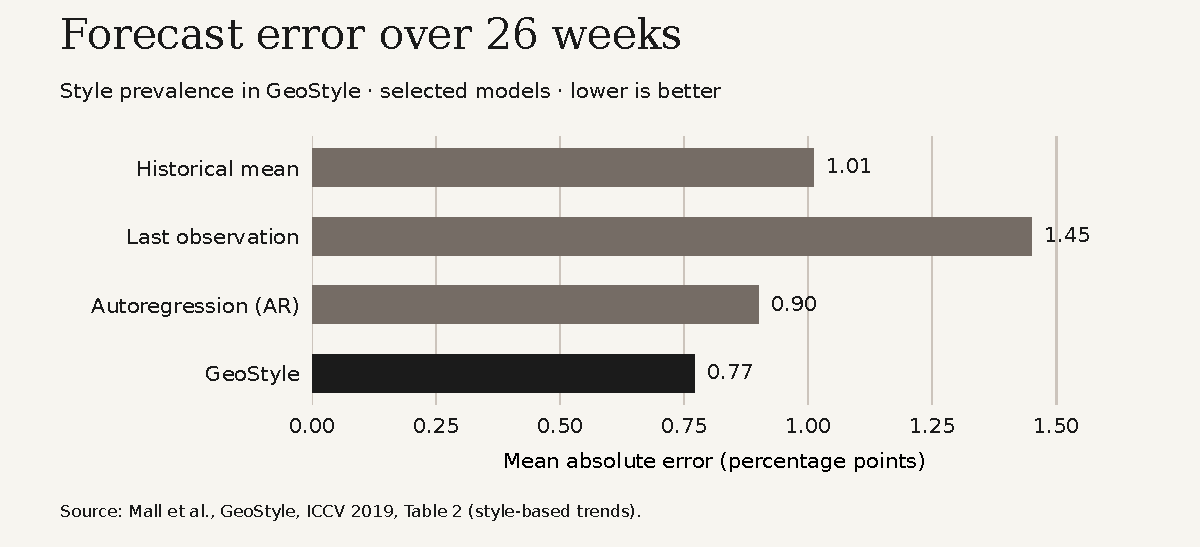
\includegraphics[width=.97\linewidth]{figures/v4-chart/geostyle_mae.pdf}\hfill\strut\par

\Caption{שגיאת חיזוי שכיחות סגנונות ל־26 שבועות, בנקודות אחוז: ממוצע היסטורי 1.01, תצפית אחרונה 1.45, אוטורגרסיה 0.90, \textenglish{GeoStyle} 0.77. ערך נמוך עדיף באותו מבחן. עיבוד \textenglish{Python} מנתוני טבלה 2 במאמר. \SourceRef{6}}

{\fontsize{13.1}{19.4}\selectfont

בחירת גוון להזמנה דורשת עוד צעד. מה שנראה פופולרי בתמונות עלול להופיע שם בגלל אירוע או תמהיל החשבונות במדגם. ההחלטה על כמות דורשת גם מחיר, עיתוי ונגישות למלאי. בשביל קניינית, תחזית מועילה היא זו שעוזרת לבחור איזה סיכון לקחת ובאיזה היקף.

\par}
